\documentclass{article}
\usepackage[utf8]{inputenc}


\usepackage[margin=1.04 in]{geometry}
\usepackage[T1]{fontenc}
\usepackage{mathtools}   % loads »amsmath«
\usepackage{amssymb}
\usepackage{amsfonts}
\usepackage{amsmath}
\usepackage{amsthm}
\usepackage{xcolor}
\usepackage{cancel}
%\usepackage{graphics}
\usepackage{graphicx}
%others
\usepackage{enumerate}
\usepackage{subcaption}



\usepackage{apacite}
\usepackage[round]{natbib}
%\bibliographystyle{plainnat}
\bibliographystyle{apacite}

\DeclarePairedDelimiter{\ceil}{\lceil}{\rceil}

\setlength{\parskip}{0.6em}
\usepackage{setspace}
\spacing{1.16}


\newtheorem{defin}{Definition.}
\newtheorem{teo}{Theorem. }
\newtheorem{lema}{Lemma. }
\newtheorem{coro}{Corolary. }
\newtheorem{prop}{Proposition. }
\theoremstyle{definition}
\newtheorem{examp}{Example. }
\newtheorem{problem}{}


\title{Problem Set 3}
\author{Giselle Labrador Badía}
\date{November 2021}

\begin{document}

\maketitle

\section*{Part 1 Nevo's code}

\subsection*{Question 1}

The results from regressions for the OLS, and IV with and without fixed effects are reported in table \ref{tab:1}. The estimates are obtained using code written in R that can be found attached. 

Now, we will briefly discuss the results. As we expected, the smaller price coefficient is the one obtained through the OLS regression. This is because endogeneity biased the price positively, that is, it underestimates the size of the effect. The mechanism in place works through demand elasticity, so an IV regression gives us a less biased coefficient. Moreover, accounting for brand fixed effect gets us closer to the real effect, since we are identifying through variation between more similar products, and substitution occurs more naturally now. The biggest and best specification is thus the IV with brand fixed effects.
% latex table generated in R 4.1.1 by xtable 1.8-4 package
% Sun Oct 31 23:15:28 2021



\begin{table}[h]
\begin{center}
\begin{tabular}{l c c c c}
\hline
 & OLS & OLS-FE & IV & IV-FE \\
\hline
(Intercept)     & $-3.60^{***}$ &                & $-3.44^{***}$ &                \\
                & $(0.11)$      &                & $(0.11)$      &                \\
price           & $-7.16^{***}$ & $-28.71^{***}$ & $-8.39^{***}$ & $-29.60^{***}$ \\
                & $(0.82)$      & $(0.93)$       & $(0.83)$      & $(0.94)$       \\

\hline
R$^2$           & $0.03$        & $0.48$         & $0.03$        & $0.29$         \\
Adj. R$^2$      & $0.03$        & $0.45$         & $0.03$        & $0.29$         \\
Num. obs.       & $2256$        & $2256$         & $2256$        & $2256$         \\
\hline
\multicolumn{5}{l}{\scriptsize{$^{***}p<0.001$; $^{**}p<0.01$; $^{*}p<0.05$}}
\end{tabular}
\caption{Regressions results for first question}
\label{tab:1}
\end{center}
\end{table}

\subsection*{Question 2}

To compute the markups and marginal costs we use the following function of partial derivartives:
\begin{equation*}
  \hat{\Omega}=\left\{\begin{array}{cc}
-\frac{\partial s_{j t}}{\partial p_{r t}} & \text { if } f \text { produces } j \text { and } r \\
0 & \text { otherwise }
\end{array}\right.  
\end{equation*}

Where $s$ is the vector of market shares for each brand in each quarter and city, and

The marginal cost and markups are therefore given by the equations
\begin{equation*}
    \hat{b}=\hat{\Omega}^{-1} \hat{s}_{j} 
\end{equation*}
$$
\text{mc}_{j}=p_{j}-\hat{b}_{j},
$$

Table 2 shows the markups and marginal costs implied by the different models. Marginal cost and markups are lower or higher respectively in models where price endogeneity is not taken care of, resulting in overestimated values. 

\begin{table}[h]
\begin{center}
\begin{tabular}{rcccc} 
\hline
& OLS & OLS-FE & IV & IV-FE \\
\hline
\mathbb{E}\left[price\right] & 0.121 & 0.121 & 0.121 & 0.122 \\
\operatorname{Med}\left(price\right) & 0.119 & 0.119 & 0.119 & 0.120 \\
sd\left(price\right) & 0.011 & 0.021 & 0.024 & 0.003 \\
\hline
\mathbb{E}\left[share\right] & 0.017 & 0.23 & 0.019 & 0.022 \\
\operatorname{Med}\left(share\right) & 0.018 & 0.012 & 0.018 & 0.014 \\
sd\left(share\right) & 0.004 & 0.002 & 0.001 & 0.002 \\
\hline
\end{tabular}
\caption{Markups and marginal costs tables}
\end{center}
\label{tab:mk}
\end{table}


 
\subsection*{Question 3}

To compute the new equilibrium prices and quantities we find a vector $p$ such that 
$$p = mc + \Omega^{-1}(p) s(p)$$
where $mc$ are marginal costs. This means finding the fixed point $p$. So with an initial price vector, we change $\Omega$ so that it reflects the merger, then we calculate a new price and update shares using the previous expression. Then, we compare these two prices and begin again if they are not close enough.
The results for post-merger places are shown in the two tables below. 
\begin{table}[h]
\begin{center}
\begin{tabular}{rcccc} 
\hline
& OLS & OLS-FE & IV & IV-FE \\
\hline
\mathbb{E}\left[price\right] & 0.121 & 0.122 & 0.123 & 0.124 \\
\operatorname{Med}\left(price\right) & 0.119 & 0.119 & 0.119 & 0.120 \\
sd\left(price\right) & 0.011 & 0.021 & 0.024 & 0.003 \\
\hline
\mathbb{E}\left[share\right] & 0.019 & 0.023 & 0.019 & 0.022 \\
\operatorname{Med}\left(share\right) & 0.018 & 0.012 & 0.018 & 0.014 \\
sd\left(share\right) & 0.004 & 0.002 & 0.001 & 0.002 \\
\hline
\end{tabular}
\caption{GM-Quaker Merger}
\end{center}
\label{tab-gmquaker}
\end{table}



\begin{table}[h]
\begin{center}
\begin{tabular}{rcccc} 
\hline
& OLS & OLS-FE & IV & IV-FE \\
\hline
\mathbb{E}\left[price\right] & 0.121 & 0.122 & 0.123 & 0.123 \\
\operatorname{Med}\left(price\right) & 0.114 & 0.119 & 0.119 & 0.110 \\
sd\left(price\right) & 0.011 & 0.021 & 0.024 & 0.003 \\
\hline
\mathbb{E}\left[share\right] & 0.017 & 0.021 & 0.018 & 0.021 \\
\operatorname{Med}\left(share\right) & 0.015 & 0.012 & 0.017 & 0.013 \\
sd\left(share\right) & 0.004 & 0.002 & 0.001 & 0.002 \\
\hline
\end{tabular}
\caption{Post-Nabisco Merger}
\end{center}
\label{tab:post-nabisco}
\end{table}



\subsection*{Question 4}
The first evident problem is that we are using the marginal costs and markups from pre-merger data. We can jointly estimate the demand to alleviate this issue. Furthermore, marginal costs can change, potentially decreasing after a merger because the merged firms become more efficient. We are also assuming that after the merger, consumers do not care about the merger, and preferences do not change. This can be due to advertising changes, or different placement of products. Also, merged firms make decisions and can alter the products of a firm and the cities in which the product is sold. Allowing for endogenous product characteristics, like mushy or sugary, could be a path to address this potential problem. 

\subsection*{Question 5}

We will use now a random coefficient model to deal with all the previous issues and captures.
\begin{table}[h]
    \centering
\begin{tabular}{rcccccc} 
\hline 
& mean & $\Sigma$ & income & income $^{2}$ & age &  child \\
\hline & & & & & & \\
constant & $-1.866$ & $0.377$ & $3.089$ & $0.000$ & $1.186$ & $0.000$ \\
& $(0.257)$ & $(0.130)$ & $(1.007)$ & $(0.000)$ & $(1.005)$ & $(0.000)$ \\
price & $-32.434$ & $1.848$ & $16.598$ & $-0.659$ & $0.000$ & $11.624$ \\
& $(7.746)$ & $(1.081)$ & $(172.930)$ & $(8.987)$ & $(0.000)$ & $(5.171)$ \\
sugar & $0.144$ & $-0.004$ & $-0.193$ & $0.000$ & $0.030$ & $0.000$ \\
& $(0.257)$ & $(0.012)$ & $(0.040)$ & $(0.000)$ & $(0.034)$ & $(0.000)$ \\
mushy & $0.832$ & $0.081$ & $1.468$ & $0.000$ & $-1.514$ & $0.000$ \\
& $(0.013)$ & $(0.207)$ & $(0.696)$ & $(0.000)$ & $(1.095)$ & $(0.000)$\\
\hline 
& GMM objective: &$14.901$\\
& $\operatorname{MD} R^{2}: $ &$0.265$\\
&$\mathrm{MD}$ weighted $R^{2}:$&$ 0.096$\\
\hline & & & & & & \\
\end{tabular}
    \caption{ BLP results}
    \label{tab:my_label}
\end{table}


\subsection*{Question 6 and 7}

Markups and marginal costs are now more precise, markups are smaller, and mean marginal costs are closer to the IV with a fixed effect model. To solve for marginal costs and markups now we use heterogeneous coefficient $\alpha_i$ that depends on $\Pi$, $\Sigma$, demographics, and product characteristics.

To find the equilibrium prices and shares post-merger we use the same equation that in 3, but this time we update computing the choice probabilities and the mean utilities that depend on the coefficients. The choice probabilities take the logit form and depend on the estimates of $\delta_{jt}$ and $\mu_{ijt}$. We compute market shares by averaging probability choices, and then predict markups using the same equation as before, but with the $\Omega$ post-merger. Repeat the process until convergence of prices. We see that the models underestimated the new equilibrium prices.



\section*{Part 2 PyBLP}

Figure 1 displays the random coefficient estimates obtained using the pyBLP package. We see that this estimates differ from the one we got using our code. 
\begin{figure}[h]
\centering
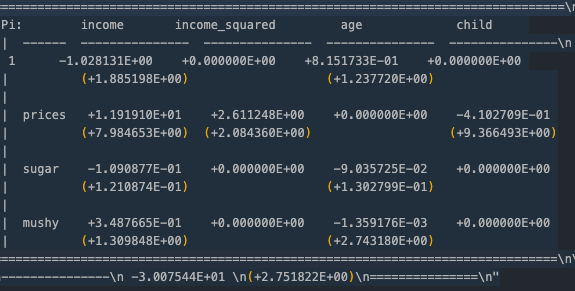
\includegraphics[width=9.5cm]{imgs/pi_py.png}
\caption{$\Pi$ coefficients of $X$ vector of characteristics.}
\end{figure}

\begin{figure}[h]
\centering
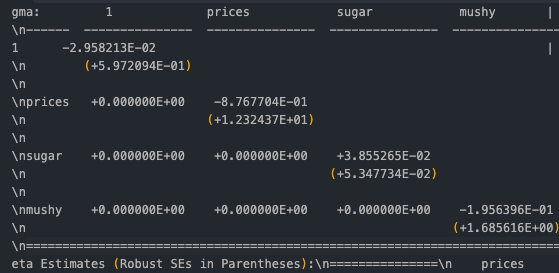
\includegraphics[width=9.5cm]{imgs/sigma_py.png}
\caption{$\Sigma$ coefficients, interaction with demographics}
\end{figure}

The main part of the Python code used is below.

\begin{figure}[h]
\centering
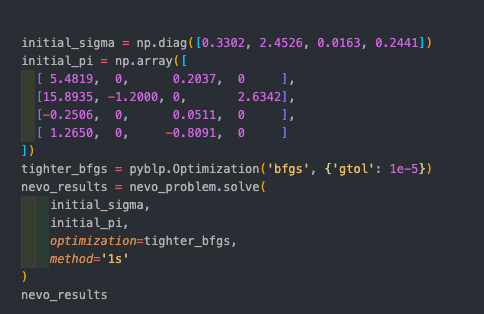
\includegraphics[width=9.5cm]{imgs/python_code.png}
\caption{Python code that calls BLP function. There is more Python code attached. }
\end{figure}

The markups and marginal costs are also different, the mean is 0.37 and 0.081 respectively, which is closer to BLP and to IV with FE. In particular, markups are strikingly greater than the ones we found.
\end{document}
